\documentclass[11pt, a4paper]{report}
% Basic Packages for Encoding (Input AND Output) and Language Support
\usepackage[utf8]{inputenc}
\usepackage[T1]{fontenc}
\usepackage[french, english]{babel}
\usepackage{lmodern}

% Importer un document externe 
\usepackage{import}
\usepackage{mdwtab}

% Packages
\import{imports/}{imports-general.tex}

% Style de pages
\import{imports/}{styles-imports.tex}

\begin{document}

\chapter*{Limitations actuelles}

De nombreux facteurs rendent l'utilisation d'ordinateurs quantiques pour le moment inutile hors de la recherche, et mêmes certains spécialistes ne sont pas convaincus qu'on arrive à passer outre afin de rendre cette technologies utilisable. Certains points sont purement liés aux algorithmes que l'on désire implémenter et qui serait potentiellement irréalisable en pratique, et d'autres concernent en général l'implémentation physique des ordinateurs quantiques, ainsi que certaines considérations purement humaine.\\ \\
Ces dernières sont les plus évidentes, et sont plus générale au sujet des nouvelles technologies. En effet, comme de nombreux autres outils électronique, tel que les téléphones portables, ordinateurs, certaines télévision récentes et ainsi de suite, les ordinateurs quantiques nécessitent dans leur fabrications actuels l'utilisation de matériaux qui sont utiles dans quantité de secteur mais ne sont pas illimité sur notre planète. Les plus évidents seront le silicium, utilisé dans n'importe quelle processeur actuel, et qui est la base de la plupart des processeur quantique actuel, comme évoqué dans la section hardware. D'autre part, l'isolation thermique d'un ordinateur quantique est généralement composé d'or (voir illustration en figure \ref{fig:photo-qc}), qui est également très prisé dans le reste de l'industrie pour ses multiples avantages d'un point de vue esthétique, thermique ou électronique.

\begin{figure}[H]
\centering
\includegraphics[width=0.7\textwidth]{qpu.eps}
\caption{Photo d'un ordinateur quantique}
\label{fig:photo-qc}
\end{figure}

De plus, une considération de l'ordre environnementale entre également en compte. Tout comme la question se pose dans le cadre de l'intelligence artificiel, l'utilisation en énergie des ordinateurs quantiques ne serait vraisemblablement pas négligeable. En effet, ils nécessitent un isolement totale ou presque du monde extérieur afin de fonctionner, ce qui demande outre l'isolation matériel évoquée plus tôt, également un refroidissement à des température proche du zéro absolu, qui est un processus très demandeur en énergie. Si l'on discute plus précisément des qubits supraconducteurs déjà présenté précédemment, il ne suffit pas juste de les mettre dans un gros congélateur, car on les contrôles depuis l'extérieur. Cela fait qu'il faut faire passer les signaux électromagnétiques depuis l'air à température ambiante jusqu'au processeur quantique au zéro absolu, tout en gardant une bonne qualité de signal. Il faut donc le refroidir petit à petit et corriger les erreurs sur le signal, tout des processus nécessitant de l'énergie et des méthode industriel de pointe pour le fabriquer.\\ \\
Il y a ensuite tout les doutes lié à la technologies à proprement parlé. Tout d'abord, comme ce fut déjà évoqué plus tôt, les ordinateurs quantiques sont soumis à beaucoup d'erreur dans les résultats dû à de multiples facteurs.

\begin{figure}[H]
\centering
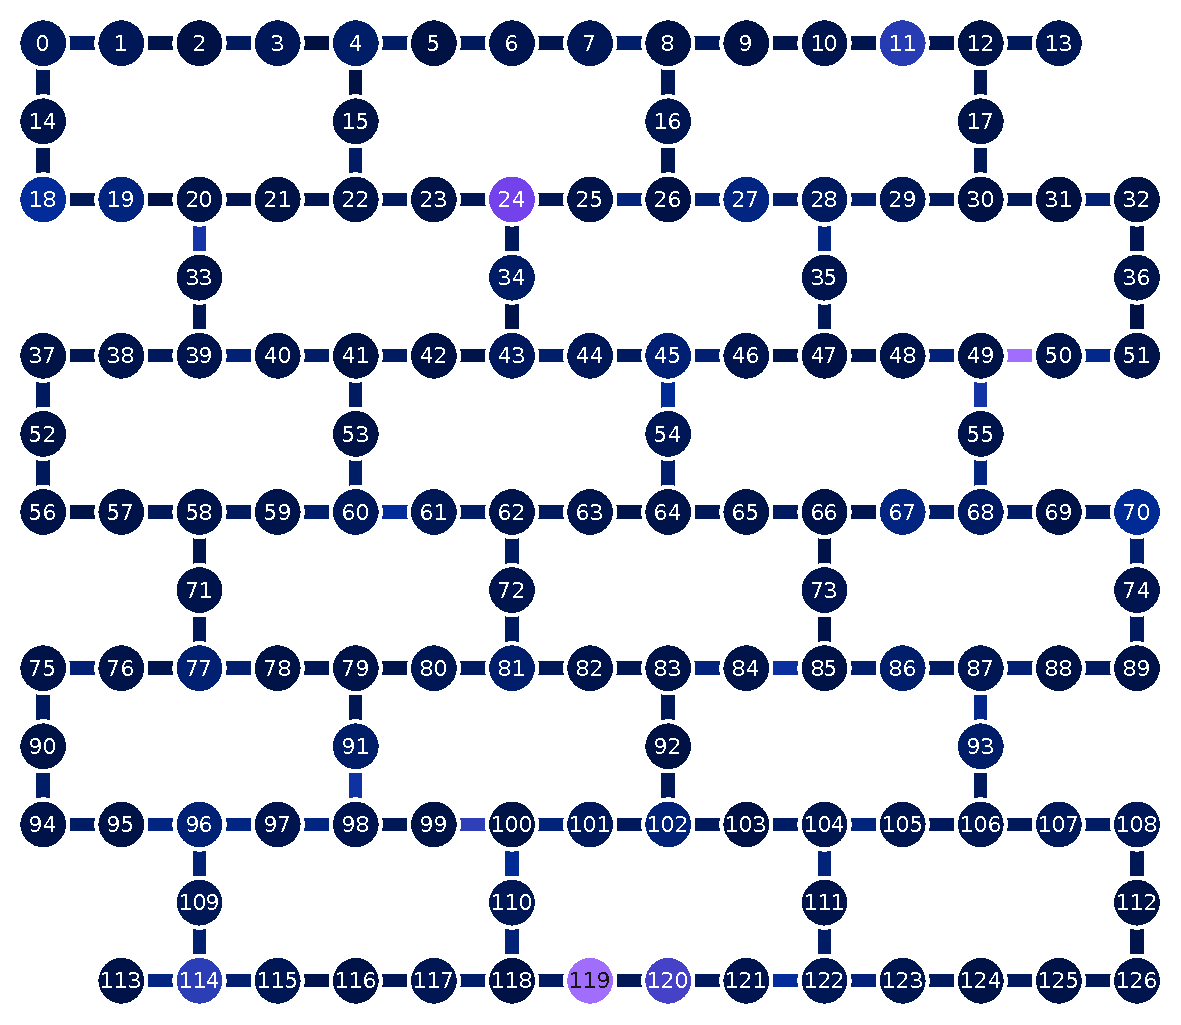
\includegraphics[width=0.7\textwidth]{ibm_brisbane_example.eps}
\caption{Exemple d'architecture d'un ordinateur quantique ($ibm\_brisbane$), les cercle représente les qubits (plus sombre est plus précis dans la mesure) et les liaisons entre eux (plus sombre a moins d'erreur sur la $CZ$)}
\label{fig:arch-qc}
\end{figure}

%%%%%%%%%%%%%%% BlaBla sur les sources d'erreur (environnement, hamiltonien, architecture) + méthode pour passer outre (surface code avec comparaison à un code classique, conception - cf. qubit du chat par exemple) %%%%%%%%%%%%%%%
Finalement, il y a les limites propre au paradigme. En effet, on suppose par exemple que la classe des problèmes solubles en temps polynomiale par un ordinateur quantique est plus grande que celle d'un ordinateur classique. Mais dire cela ainsi est quelque peut mensonger, car on considère traditionnellement comme classe polynomiale pour les ordinateurs quantiques la complexité dite $BQP$ (\textit{bounded-error quantum polynomial time}), qui signifie qu'un problème peut être résolu dans un temps polynomial avec une erreur inférieur à $\frac{1}{3}$. Il existe un groupe de complexité similaire pour les ordinateurs classiques, nommée $BPP$ (\textit{bounded-error probabilistic polynomial time}), mais elle est moins intéressante car c'est un système bien déterminé et demeure selon nos connaissances actuels une moins grande catégorie de problèmes.\\
L'algorithme de Shor est un bon exemple d'un problème qui n'est vraisemblablement pas dans $P$ (temps polynomial) mais qui est dans $BQP$. Comme on a vu avec celui-ci, on n'est pas certain d'obtenir le bon résultat à la mesure, ce qui fait que par manque de chance, en pratique, cela pourrait prendre plus de temps qu'un algorithme en général plus lent mais qui donne à coup sûr la solution escomptée. Si l'on rajoute ce qui a été discuté plus haut au sujet du bruit et des erreurs, cela rend les ordinateurs quantiques encore plus complexe à mettre en place comme il faut trouver des applications ne subissant pas trop ces erreurs.\\
Citons encore certaines méthodes pour lesquels les ordinateurs quantiques peuvent être avantageux, comme pour du \textit{machine learning}, où pour bénéficier d'une accélération le circuit doit être assez grand. Néanmoins plus le circuit grandit, plus la préparation de l'état du système quantique nécessaire à la réalisation de l'algorithme devient compliqué et remet donc en question l'avantage. On arrive donc à un cercle vicieux pour lequel l'avantage est incertain, car plus le problème est gros plus l'avantage est conséquent, mais plus la mise en place est compliquée et en réduit quelque peu l'intérêt.\\ \\
En résumé, il n'y a encore aucune certitude sur la viabilité de la technologie, même si il y a de nombreux signes encourageant. Tout ces limitations présentent des défis qui devront être contourné ou outrepasser à l'avenir grâce aux débouchées de la recherche.

\end{document}